\documentclass[11pt,a4paper]{article}

\usepackage[utf8]{inputenc}
\usepackage[T1]{fontenc}
\usepackage{lmodern}
\usepackage[a4paper,margin=1.7cm]{geometry}
\usepackage{graphicx}
\usepackage{booktabs}
\usepackage{tabularx}
\usepackage{array}
\usepackage{longtable}
\usepackage{multirow}
\usepackage[table]{xcolor}
\usepackage{tikz}
\usetikzlibrary{positioning,arrows.meta}
\usepackage[most]{tcolorbox}
\usepackage{enumitem}
\usepackage{titlesec}
\usepackage{fancyhdr}
\usepackage[hyperfootnotes=false]{hyperref}
\usepackage{xurl}
\usepackage{amsmath,amssymb}
\usepackage{float}
\usepackage{caption}
\usepackage{lastpage}
\usepackage{ragged2e}
\usepackage{setspace}
\usepackage{colortbl}
\usepackage[hang,flushmargin]{footmisc}

\definecolor{navy}{HTML}{0B3954}
\definecolor{teal}{HTML}{087E8B}
\definecolor{gold}{HTML}{F4B942}
\definecolor{coral}{HTML}{FF6B35}
\definecolor{plum}{HTML}{7B2CBF}
\definecolor{slate}{HTML}{34495E}
\definecolor{softblue}{HTML}{EEF6FA}
\definecolor{softteal}{HTML}{EAF7F8}
\definecolor{softgold}{HTML}{FFF7E3}
\definecolor{softgray}{HTML}{F7FAFC}
\definecolor{linegray}{HTML}{D6DEE8}

\hypersetup{
  colorlinks=true,
  urlcolor=teal,
  linkcolor=navy,
  citecolor=plum,
  pdftitle={Pattern Recognition Final Project Proposal},
  pdfauthor={Pattern Recognition Course Project Team},
  pdfsubject={Portfolio Management, Regime Detection, Reinforcement Learning},
  pdfkeywords={Portfolio Management, Reinforcement Learning, Market Regimes, Macro Data, Financial News}
}
\urlstyle{same}
\onehalfspacing
\setlength{\parindent}{0pt}
\setlength{\parskip}{0.5em}
\renewcommand{\arraystretch}{1.2}
\emergencystretch=2em

\newcolumntype{Y}{>{\RaggedRight\arraybackslash}X}
\newcolumntype{P}[1]{>{\RaggedRight\arraybackslash}p{#1}}
\newcommand{\fncite}[2]{\footnote{#1. \url{#2}}}

\titleformat{\section}{\Large\bfseries\color{navy}}{\thesection}{0.6em}{}
\titleformat{\subsection}{\large\bfseries\color{teal}}{\thesubsection}{0.6em}{}
\titleformat{\subsubsection}{\normalsize\bfseries\color{plum}}{\thesubsubsection}{0.6em}{}
\titlespacing*{\section}{0pt}{0.6em}{0.4em}
\titlespacing*{\subsection}{0pt}{0.5em}{0.25em}

\pagestyle{fancy}
\fancyhf{}
\fancyhead[L]{\color{navy}\bfseries Pattern Recognition Final Project Proposal}
\fancyhead[R]{\color{slate}Portfolio Management}
\fancyfoot[C]{\color{slate}\thepage/\pageref{LastPage}}
\setlength{\headheight}{15pt}

\newtcolorbox{summarybox}[1][]{
  enhanced,
  colback=softblue,
  colframe=navy,
  boxrule=0.8pt,
  arc=3mm,
  left=2mm,
  right=2mm,
  top=1.5mm,
  bottom=1.5mm,
  #1
}

\newtcolorbox{insightbox}[1][]{
  enhanced,
  colback=softteal,
  colframe=teal,
  boxrule=0.8pt,
  arc=3mm,
  left=2mm,
  right=2mm,
  top=1.5mm,
  bottom=1.5mm,
  #1
}

\newtcolorbox{warningbox}[1][]{
  enhanced,
  colback=softgold,
  colframe=gold!70!black,
  boxrule=0.8pt,
  arc=3mm,
  left=2mm,
  right=2mm,
  top=1.5mm,
  bottom=1.5mm,
  #1
}

\begin{document}

\hypersetup{pageanchor=false}
\begin{titlepage}
\begin{tikzpicture}[remember picture,overlay]
  \fill[navy] (current page.north west) rectangle ([yshift=-7.8cm]current page.north east);
  \fill[teal] (current page.south west) rectangle ([yshift=1.6cm]current page.south east);
  \fill[gold,opacity=0.95] ([xshift=-1.8cm,yshift=-1.2cm]current page.north east) circle (1.85cm);
  \fill[coral,opacity=0.88] ([xshift=1.4cm,yshift=-3.0cm]current page.north west) circle (1.2cm);
\end{tikzpicture}

\vspace*{1.4cm}

{\color{white}\sffamily\bfseries\fontsize{24}{28}\selectfont
News-Augmented\\[0.12em]
Market Regime Detection\\[0.12em]
for Reinforcement Learning ETF Allocation\par}

\vspace{0.8cm}

{\color{white}\Large\sffamily Detailed Project Proposal for a Pattern Recognition Course Final Project\par}

\vspace{0.6cm}

{\color{white}\large\sffamily Portfolio Management Focus, 6-Student Team, 1-Month Delivery Horizon\par}

\vspace{1.3cm}

\begin{summarybox}[width=\textwidth,colback=white,colframe=white]
\textbf{\color{navy}Executive Positioning.}
This proposal frames the project as a \textbf{pattern-recognition-first} portfolio management system.
The central technical contribution is a market regime model learned from quantitative market data, compact macro data, and structured news factors.
Reinforcement learning is used as a downstream decision layer to test whether the learned regime representation improves ETF allocation quality.
\end{summarybox}

\vspace{0.5cm}

\begin{tabularx}{\textwidth}{@{}P{0.22\textwidth}Y@{}}
\textbf{\color{navy}Submission Date} & March 23, 2026 \\
\textbf{\color{navy}Primary Data Window} & January 2, 2014 to March 20, 2026 \\
\textbf{\color{navy}Core Tradable Assets} & SPY, TLT, GLD, with cash as an action option \\
\textbf{\color{navy}Context Indicators} & QQQ, \^VIX, and \^TNX as state variables rather than direct allocation targets \\
\textbf{\color{navy}Main Regime Model} & Gaussian HMM on fused weekly state features \\
\textbf{\color{navy}Main RL Design} & Weekly discrete-allocation agent with transaction-cost-aware reward \\
\end{tabularx}

\vfill

{\color{white}\large\sffamily Prepared for submission as a course project proposal\par}
\end{titlepage}
\clearpage
\pagenumbering{arabic}
\hypersetup{pageanchor=true}

\tableofcontents
\newpage

\section{Executive Summary}

This project addresses a common weakness in financial machine learning proposals: too much ambition at the data and model level, but not enough attention to feasibility, alignment, and evaluation.
The team initially considered a broad multimodal system combining full macro-economic databases, market prices, financial news, large language models, and reinforcement learning.
That full design is too wide for a 1-month implementation window.

The proposed final scope is intentionally narrower and stronger:

\begin{itemize}[leftmargin=1.4em]
  \item \textbf{Primary historical system:} price plus macro regime detection for a full historical backtest.
  \item \textbf{Qualitative extension:} news-derived sentiment and topic factors as a recent-window overlay and explanation aid.
  \item \textbf{Decision layer:} a weekly reinforcement learning allocator that chooses among a small set of interpretable ETF allocation templates.
  \item \textbf{Explanation layer:} an auxiliary LLM-based summarizer that explains the learned regime and the portfolio action without replacing the numerical model.
\end{itemize}

\begin{summarybox}[title=\textbf{Proposal At a Glance}]
\begin{itemize}[leftmargin=1.4em]
  \item \textbf{Research question:} Can latent market regimes learned from quantitative and qualitative factors improve ETF allocation quality relative to price-only decision-making?
  \item \textbf{Main scientific contribution:} discovery of interpretable latent market states from fused price, macro, and text features.
  \item \textbf{Main engineering contribution:} a clean weekly state pipeline that aligns mixed-frequency macro data and recent financial headlines with market data.
  \item \textbf{Main practical contribution:} a reproducible backtesting framework that is explainable, scope-controlled, and robust enough to finish on time.
\end{itemize}
\end{summarybox}

\section{Motivation and Problem Statement}

Portfolio management is a natural application domain for pattern recognition because financial markets generate large, noisy, temporally dependent data streams.
However, many financial reinforcement learning systems still suffer from two major problems:

\begin{itemize}[leftmargin=1.4em]
  \item \textbf{Overfitting to historical noise.} Flexible policies can exploit spurious patterns that do not generalize.
  \item \textbf{Lack of interpretability.} Pure black-box systems can produce portfolio actions without an understandable account of the market state.
\end{itemize}

This proposal addresses both issues by separating the problem into two layers:

\begin{enumerate}[leftmargin=1.5em]
  \item a \textbf{pattern recognition layer} that learns compact and interpretable market regimes, and
  \item a \textbf{reinforcement learning layer} that uses those regimes to make allocation decisions.
\end{enumerate}

This decomposition makes the project more defensible in a pattern recognition course.
The regime model is deliberately a \emph{classical pattern recognition} object: a latent-variable sequential model that detects recurring structures in noisy multivariate observations rather than directly predicting actions.
The central claim is not ``we trained an RL trader.''
The central claim is:

\begin{summarybox}
\centering
\textbf{\color{navy}A structured market-state representation learned from prices, macro conditions, and news context can improve downstream portfolio decisions while remaining more interpretable than a monolithic RL policy.}
\end{summarybox}

\section{Objectives, Scope, and Hypotheses}

\subsection{Project Objectives}

\begin{itemize}[leftmargin=1.4em]
  \item Build a compact, aligned, multimodal financial dataset suitable for portfolio management.
  \item Learn latent market regimes from fused quantitative and qualitative features.
  \item Test whether regime-aware reinforcement learning outperforms price-only reinforcement learning and standard portfolio baselines.
  \item Provide human-readable explanations of regime changes and portfolio actions without making the LLM the sole decision-maker.
\end{itemize}

\subsection{Hypotheses}

\begin{enumerate}[leftmargin=1.5em]
  \item \textbf{H1:} Price plus macro features will produce more stable and economically meaningful market regimes than price features alone.
  \item \textbf{H2:} Adding structured news factors will improve recent-window regime interpretation and provide qualitatively consistent market context, even if they are not yet available over the entire historical backtest horizon.
  \item \textbf{H3:} Regime-aware RL will yield better risk-adjusted performance than price-only RL and simple static baselines.
  \item \textbf{H4:} A separated explanation layer can produce narratives that are consistent with the quantitative regime assignments without replacing the numerical model.
\end{enumerate}

\subsection{Hypothesis-to-Evidence Map}

\begin{table}[H]
\centering
\caption{What will count as evidence for each main claim}
\begin{tabularx}{\textwidth}{@{}P{0.16\textwidth}Y@{}}
\toprule
\rowcolor{softteal}
\textbf{Claim} & \textbf{Main evidence in the final report} \\
\midrule
H1 & Regime stability, transition coherence, and economically sensible episode assignments for \textbf{price-only} versus \textbf{price+macro} models \\
H2 & Recent-window case study, manually reviewed Yahoo headline labels, and explanation consistency checks \\
H3 & Comparison against static baselines, a regime-aware heuristic allocator, price-only RL, and regime-aware RL \\
H4 & Manual alignment review of explanation outputs on sampled weeks using the model's actual supporting signals \\
\bottomrule
\end{tabularx}
\end{table}

\subsection{Scope Control}

\begin{warningbox}[title=\textbf{Explicit Scope Control}]
\begin{itemize}[leftmargin=1.4em]
  \item \textbf{Included:} lag-aware macro panel, small ETF universe, weekly RL, structured headline factors, interpretable action templates.
  \item \textbf{Excluded from the main submission:} full FRED-MD preprocessing, raw full-text news scraping, complex memory-based LLM agents, and continuous-action RL as the first benchmark.
\end{itemize}
\end{warningbox}

\section{Data Assets, Coverage, and Alignment}

\subsection{Collected Data Sources}

\begin{table}[H]
\centering
\caption{Project data assets and their intended role}
\begin{tabularx}{\textwidth}{@{}P{0.16\textwidth}P{0.17\textwidth}P{0.17\textwidth}P{0.12\textwidth}Y@{}}
\toprule
\rowcolor{softblue}
\textbf{Block} & \textbf{Source} & \textbf{Current Coverage} & \textbf{Raw Frequency} & \textbf{Role in the Project} \\
\midrule
Price data & Yahoo Finance via \texttt{yfinance} & 2014-01-02 to 2026-03-20 & Daily trading days & Core market features, returns, volatility, and tradable asset history \\
Macro panel & FRED official CSV downloads & Multi-decade history, latest values mostly through March 2026 & Daily, weekly, monthly mixed & Regime context, macro stress, rates, inflation expectations, and slow macro confirmation \\
News metadata & Yahoo Finance via \texttt{get\_news()} & 2026-03-04 to 2026-03-23 & Event-driven & Recent sentiment, topic, relevance, and live-market context \\
Text sanity set & Financial PhraseBank & Static corpus & Sentence-level labeled text & Sentiment pipeline validation only; not the main trading dataset \\
\bottomrule
\end{tabularx}
\end{table}

Historical market data are collected through the \texttt{yfinance} interface\fncite{Ran Aroussi, \emph{yfinance} documentation}{https://ranaroussi.github.io/yfinance/index.html} and the macro panel is pulled from official FRED endpoints published by the Federal Reserve Bank of St.~Louis\fncite{Federal Reserve Bank of St.~Louis, FRED API overview}{https://fred.stlouisfed.org/docs/api/fred/overview.html}. The optional text sanity set is based on Financial PhraseBank and related financial sentiment literature\fncite{Pekka Malo et al., \emph{Good Debt or Bad Debt: Detecting Semantic Orientations in Economic Texts}, 2013}{https://arxiv.org/abs/1307.5336}.

In this proposal, \emph{tradable assets} are the instruments that receive portfolio weights directly, namely SPY, TLT, and GLD. By contrast, QQQ, \^VIX, and \^TNX are treated as \emph{context indicators}: they enter the state representation but are not direct allocation targets. On the macro side, the current frozen working snapshot is a compact 10-series panel, while the collection script also supports a broader 16-series \emph{core} preset for the next expansion round.

\subsection{Exact Data Fields to Keep}

\begin{table}[H]
\centering
\caption{Field-level schema retained for modeling}
\begin{tabularx}{\textwidth}{@{}P{0.18\textwidth}Y@{}}
\toprule
\rowcolor{softteal}
\textbf{Source} & \textbf{Fields retained} \\
\midrule
Price table & \texttt{date, symbol, open, high, low, close, adj\_close, volume, source} \\
Macro table & \texttt{date, series\_id, value, category, frequency, description, suggested\_transform, source} \\
News table & \texttt{requested\_symbol, news\_id, content\_type, title, summary, published\_at, publisher, canonical\_url, click\_url, related\_tickers, query\_relevance\_heuristic, source} \\
Derived weekly state & \texttt{week\_end, X\_price, X\_macro, X\_text, regime\_posterior, previous\_weights, next\_period\_returns} \\
\bottomrule
\end{tabularx}
\end{table}

The field \texttt{query\_relevance\_heuristic} is a transparent rule-based pre-filter, not a learned model. It should be documented as a simple combination of ticker matching, related-symbol matching, and macro-keyword matching.

\begin{figure}[H]
\centering
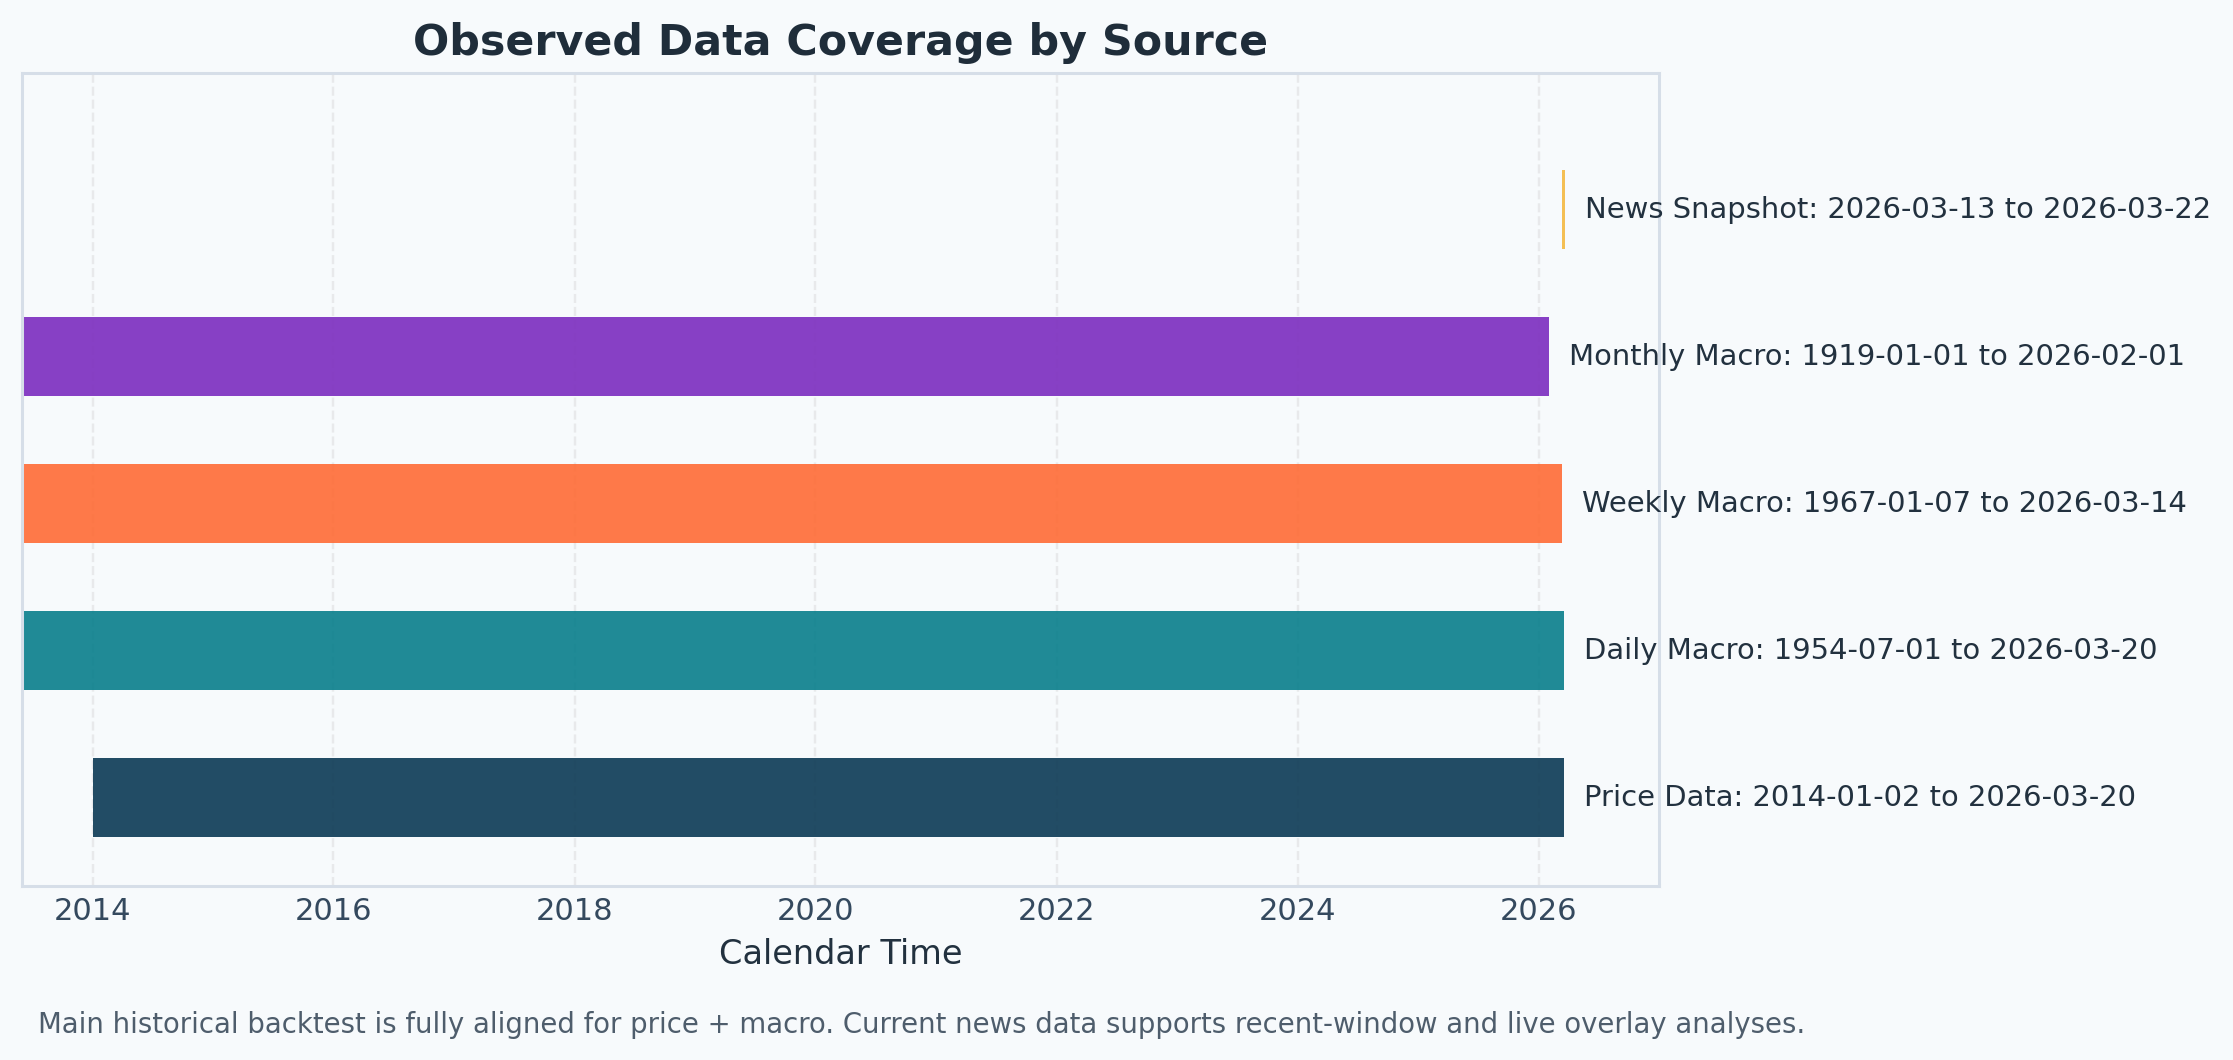
\includegraphics[width=\textwidth]{assets/data_coverage_timeline.png}
\caption{Observed coverage by source as of March 23, 2026. The long historical window is already available for price plus macro modeling. News currently supports recent-window and live-overlay experiments.}
\end{figure}

\subsection{Temporal Coverage and Alignment Logic}

The collected data does \emph{not} align naturally in its raw form.
Prices are daily, macro series are mixed daily/weekly/monthly, and news arrives irregularly.
Therefore, the modeling calendar must be defined independently of the raw data frequency.

\begin{insightbox}[title=\textbf{Alignment Strategy}]
\begin{enumerate}[leftmargin=1.5em]
  \item Engineer rolling price features on a daily calendar.
  \item Resample macro features to the weekly decision calendar.
  \item Lag weekly macro signals by one week.
  \item Lag monthly macro signals by one month.
  \item Aggregate news events into weekly text factors.
  \item Join all blocks into one weekly state vector used by both the regime model and the RL environment.
\end{enumerate}
\end{insightbox}

This lagging rule is a conservative approximation rather than a full publication-calendar model. A more exact implementation would track release timestamps, for example through ALFRED-style vintages, but that is outside the scope of this course project.

\subsection{What Is Fully Aligned Right Now}

\begin{itemize}[leftmargin=1.4em]
  \item \textbf{Price plus macro:} fully usable for the main historical project window from January 2, 2014 to March 20, 2026.
  \item \textbf{Price plus macro plus text:} not yet fully historical because current Yahoo headline extraction covers only about 18.8 days.
\end{itemize}

This means the main backtest should be built around \textbf{price plus macro} and the qualitative block should be positioned as:

\begin{itemize}[leftmargin=1.4em]
  \item a recent-window ablation,
  \item a recent live overlay, and
  \item an explanation and context module.
\end{itemize}

\begin{warningbox}[title=\textbf{Reproducibility Notes}]
\begin{itemize}[leftmargin=1.4em]
  \item Yahoo \texttt{adj\_close} can change over time because dividend and split adjustments propagate retroactively.
  \item Yahoo news feeds are recent and mutable rather than archival.
  \item The report should therefore treat the current CSV files as a frozen experiment snapshot.
\end{itemize}
\end{warningbox}

\section{Proposed System Architecture}

\begin{figure}[H]
\centering
\resizebox{\textwidth}{!}{%
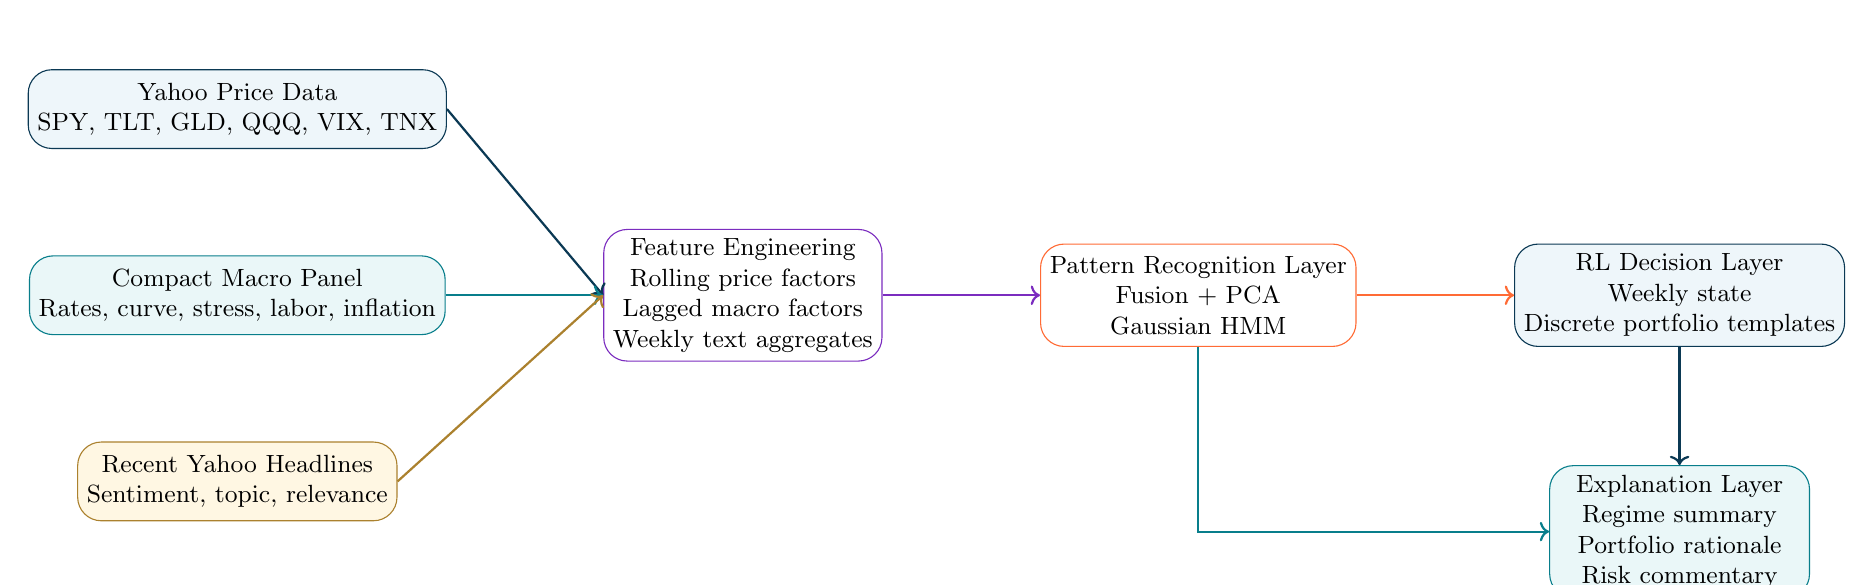
\begin{tikzpicture}[node distance=1.35cm and 0.8cm, every node/.style={font=\small}]
  \node[draw=navy, fill=softblue, rounded corners=3mm, minimum width=3.2cm, minimum height=1.0cm, align=center] (prices) {Yahoo Price Data\\SPY, TLT, GLD, QQQ, VIX, TNX};
  \node[draw=teal, fill=softteal, rounded corners=3mm, minimum width=3.2cm, minimum height=1.0cm, align=center, below=of prices] (macro) {Compact Macro Panel\\Rates, curve, stress, labor, inflation};
  \node[draw=gold!70!black, fill=softgold, rounded corners=3mm, minimum width=3.2cm, minimum height=1.0cm, align=center, below=of macro] (news) {Recent Yahoo Headlines\\Sentiment, topic, relevance};

  \node[draw=plum, fill=white, rounded corners=3mm, minimum width=3.3cm, minimum height=1.3cm, align=center, right=2.0cm of macro] (features) {Feature Engineering\\Rolling price factors\\Lagged macro factors\\Weekly text aggregates};
  \node[draw=coral, fill=white, rounded corners=3mm, minimum width=3.3cm, minimum height=1.3cm, align=center, right=2.0cm of features] (regime) {Pattern Recognition Layer\\Fusion + PCA\\Gaussian HMM};
  \node[draw=navy, fill=softblue, rounded corners=3mm, minimum width=3.3cm, minimum height=1.3cm, align=center, right=2.0cm of regime] (rl) {RL Decision Layer\\Weekly state\\Discrete portfolio templates};
  \node[draw=teal, fill=softteal, rounded corners=3mm, minimum width=3.3cm, minimum height=1.3cm, align=center, below=1.5cm of rl] (xai) {Explanation Layer\\Regime summary\\Portfolio rationale\\Risk commentary};

  \draw[->, thick, color=navy] (prices.east) -- (features.west);
  \draw[->, thick, color=teal] (macro.east) -- (features.west);
  \draw[->, thick, color=gold!70!black] (news.east) -- (features.west);
  \draw[->, thick, color=plum] (features.east) -- (regime.west);
  \draw[->, thick, color=coral] (regime.east) -- (rl.west);
  \draw[->, thick, color=teal] (regime.south) |- (xai.west);
  \draw[->, thick, color=navy] (rl.south) -- (xai.north);
\end{tikzpicture}
}
\caption{Proposed architecture. The numerical model remains the core decision engine; the explanation layer is added for interpretability and presentation quality.}
\end{figure}

In implementation, the train/validation/test barrier is enforced before any scaler, PCA transform, HMM fit, or RL policy fit is estimated. The highest leakage risk is in feature engineering and latent-state estimation, so these stages must remain strictly causal.

\section{Pattern Recognition Layer}

\subsection{Model-Ready Weekly State}

For each weekly rebalancing date $t$, the project constructs three feature blocks:

\begin{align*}
X_{\text{price}}^{(t)} &= \text{recent market features from daily OHLCV and cross-asset behavior}, \\
X_{\text{macro}}^{(t)} &= \text{lagged macro-financial variables known by time } t, \\
X_{\text{text}}^{(t)} &= \text{weekly headline aggregates such as sentiment and topic intensity}.
\end{align*}

The fused weekly feature row is then:
\[
x_t = \left[X_{\text{price}}^{(t)},\; X_{\text{macro}}^{(t)},\; X_{\text{text}}^{(t)}\right].
\]

\subsection{Quantitative Feature Block}

The quantitative block should be the backbone of the project.
It is stable, observable, and available over a sufficiently long historical horizon.

\subsubsection{Price-Derived Features}

\begin{itemize}[leftmargin=1.4em]
  \item 1-day, 5-day, and 20-day log returns
  \item realized volatility over 5 and 20 trading days
  \item rolling drawdown
  \item moving-average gaps
  \item intraday range proxy
  \item volume z-score
  \item relative strength such as QQQ/SPY
  \item rolling correlations such as corr(SPY, TLT) and corr(SPY, GLD)
  \item VIX level and short-horizon change
  \item TNX level and short-horizon change
\end{itemize}

\subsubsection{Macro-Derived Features}

\begin{itemize}[leftmargin=1.4em]
  \item federal funds level and short-horizon change
  \item 10-year yield level and change
  \item yield curve slope and sign
  \item breakeven inflation level and change
  \item financial conditions level and delta
  \item initial jobless claims level and recent change
  \item lagged CPI, unemployment, industrial production, and consumer sentiment context
\end{itemize}

\subsubsection{Primary Encoder Choice}

For the main project, the best choice is a deterministic and interpretable encoder:

\begin{itemize}[leftmargin=1.4em]
  \item feature engineering,
  \item standardization,
  \item PCA chosen from the training sample only.
\end{itemize}

This approach has three advantages:

\begin{enumerate}[leftmargin=1.5em]
  \item it is feasible within one month,
  \item it supports clean ablations, and
  \item it is easy to explain in a course presentation.
\end{enumerate}

The project should commit in advance to keeping roughly 8--12 principal components, with the exact choice made from training-set-only diagnostics such as explained variance and HMM fit quality. This avoids leaving PCA as an ex-post degree of freedom.

\subsection{Qualitative Feature Block}

The qualitative block should \textbf{not} be treated as a generative free-text system.
Instead, it should transform headlines into structured factors.

\subsubsection{Per-Headline Labels}

Each headline should produce:

\begin{itemize}[leftmargin=1.4em]
  \item sentiment: negative, neutral, or positive,
  \item topic: growth/earnings, inflation/rates, recession/slowdown, geopolitics/policy, or market technical/flow,
  \item relevance score to the tracked asset universe,
  \item optional impact score.
\end{itemize}

\subsubsection{Text Modeling Recommendation}

The preferred pipeline is:

\begin{enumerate}[leftmargin=1.5em]
  \item rule-based relevance filtering,
  \item a lightweight financial sentiment/topic classifier,
  \item weekly aggregation.
\end{enumerate}

The best practical starting point is a FinBERT-style sentiment model or a small classifier\fncite{Dogu Araci, \emph{FinBERT: Financial Sentiment Analysis with Pre-trained Language Models}, 2019}{https://arxiv.org/abs/1908.10063}.
An LLM prompt can be used as a fallback extraction tool, but it should not be the single point of failure for the whole backtest.

Because Yahoo Finance headlines are short and noisy, the model should also be checked on a small manually labeled sample of actual Yahoo headlines rather than relying only on external benchmark corpora.

\subsubsection{Weekly Text Aggregates}

The final text features may include:

\begin{itemize}[leftmargin=1.4em]
  \item headline count,
  \item mean sentiment,
  \item negative sentiment ratio,
  \item topic proportions,
  \item maximum impact score,
  \item relevance ratio.
\end{itemize}

\subsection{Feature Fusion and Regime Discovery}

The proposal deliberately avoids heavy multimodal architectures as a first step.
Instead, it uses feature-level fusion:

\begin{enumerate}[leftmargin=1.5em]
  \item clean each block independently,
  \item standardize each block,
  \item concatenate into $x_t$,
  \item compress with PCA,
  \item train a diagonal-covariance Gaussian HMM with $K \in \{3,4\}$ latent states\fncite{James D.~Hamilton, \emph{A New Approach to the Economic Analysis of Nonstationary Time Series and the Business Cycle}, 1989}{https://www.econometricsociety.org/publications/econometrica/1989/03/01/new-approach-economic-analysis-nonstationary-time-series-and}.
\end{enumerate}

\begin{insightbox}[title=\textbf{Why HMM Is the Right First Regime Model}]
A Gaussian HMM is a classical pattern recognition model: latent-state, generative, and sequential.
It is appropriate here because financial regimes exhibit persistence and transition structure rather than independent clustering from week to week.
The Markov assumption is not perfect, but it is a reasonable first inductive bias for regime duration and regime switching in a one-month course project.
\end{insightbox}

\begin{insightbox}[title=\textbf{Why the Regime Model Matters}]
The regime model is the main scientific contribution of the project.
It converts noisy multimodal observations into a compact latent state representation that is interpretable, analyzable, and directly usable by the RL agent.
\end{insightbox}

\begin{warningbox}[title=\textbf{Parameter-Control Decision}]
Weekly data are limited, so the HMM must be protected against over-parameterization.
The project therefore commits to PCA before HMM fitting, diagonal covariance rather than full covariance, and a preference for $K=3$ unless $K=4$ is clearly justified on training and validation diagnostics.
\end{warningbox}

\subsection{Stretch Extensions}

If the baseline is stable early, the following extensions are valid:

\begin{itemize}[leftmargin=1.4em]
  \item a TCN over the recent numerical feature window,
  \item a denoising autoencoder,
  \item a VAE that produces a latent vector $z_t$ before HMM modeling.
\end{itemize}

These are explicitly \textbf{stretch goals}, not core requirements.

\subsection{Failure and Fallback Logic}

If the HMM collapses to one dominant state, produces unstable fits, or yields economically meaningless regimes, the fallback order should be:

\begin{enumerate}[leftmargin=1.5em]
  \item reduce $K$,
  \item reduce PCA dimension,
  \item switch to GMM or KMeans on the same compressed features,
  \item if necessary, use a simple rule-based volatility regime so the downstream allocator can still be evaluated.
\end{enumerate}

\begin{figure}[H]
\centering
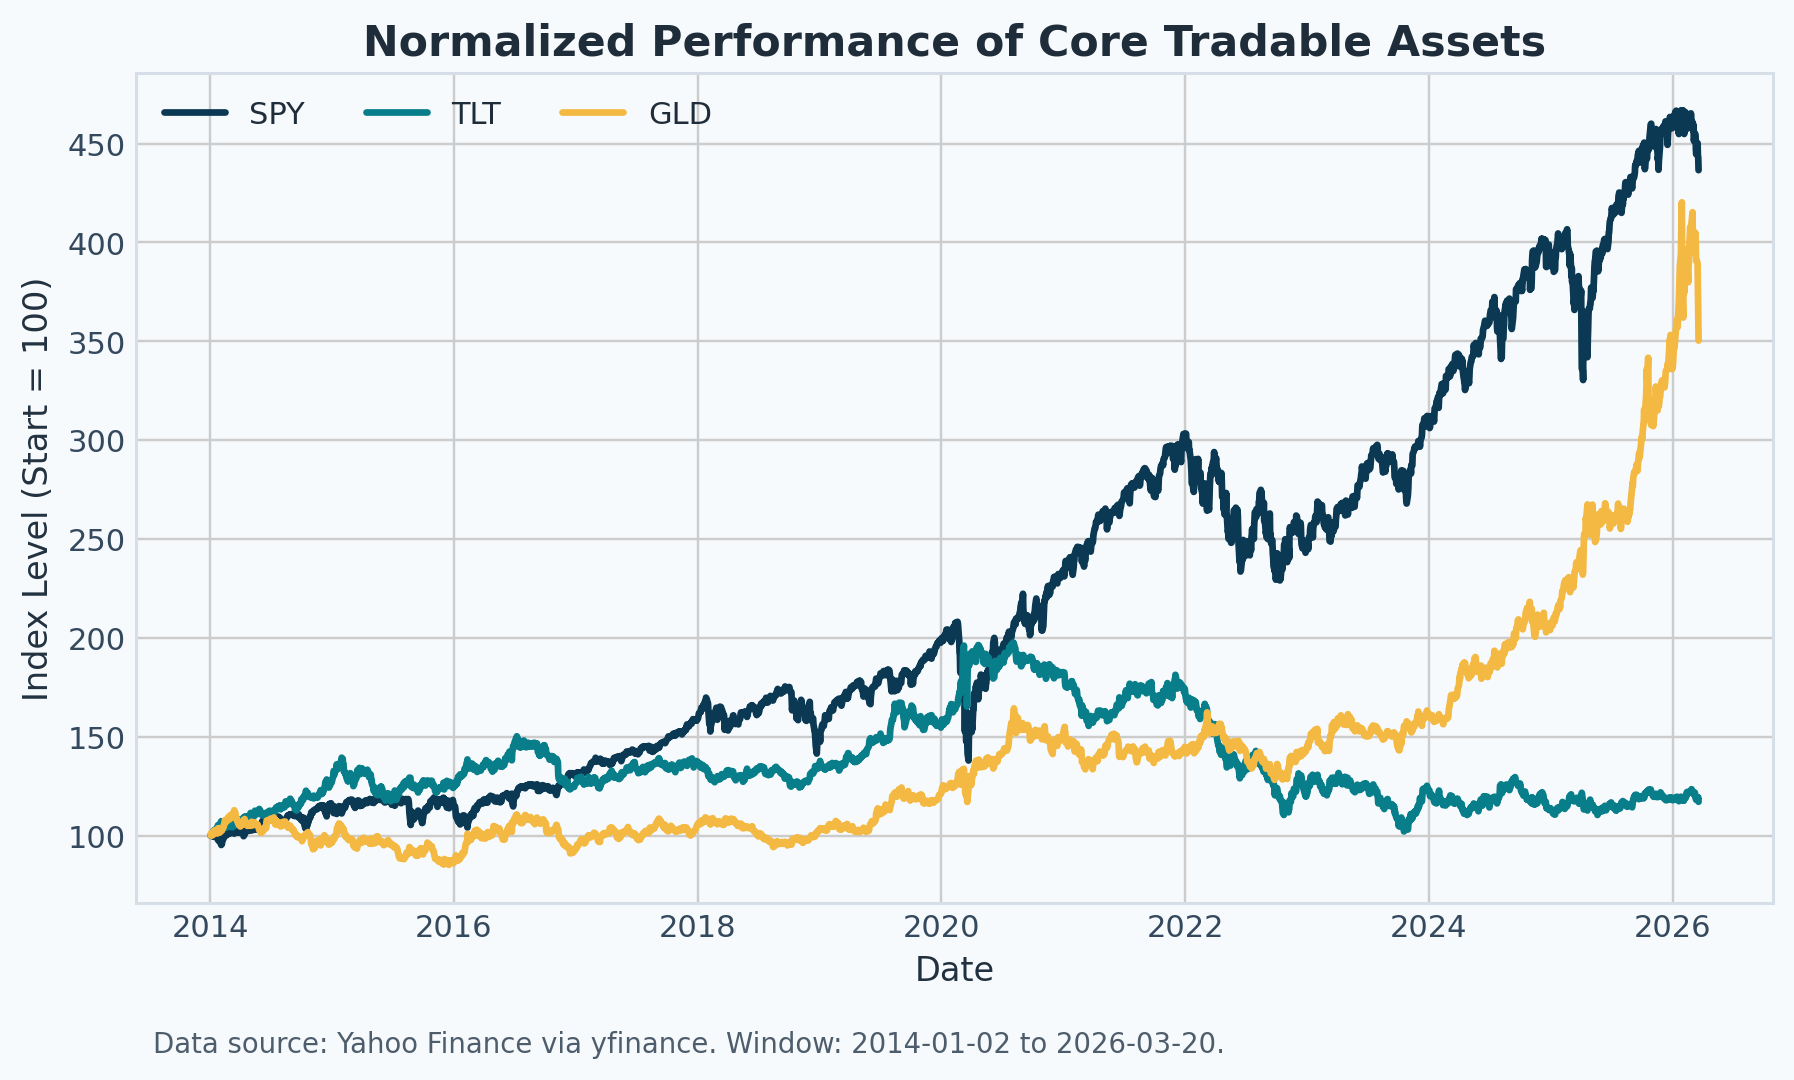
\includegraphics[width=\textwidth]{assets/normalized_assets.png}
\caption{Normalized performance of the core tradable assets used in the action space. These assets provide a compact and interpretable ETF universe for allocation experiments.}
\end{figure}

\section{Reinforcement Learning Formulation}

\subsection{Environment Design}

The RL layer operates on a \textbf{weekly rebalancing calendar}.
This choice reduces turnover, reduces sensitivity to market micro-noise, and aligns naturally with mixed-frequency macro information.

\subsection{Markov Decision Process}

\subsubsection{State}

At rebalancing step $t$, define the state as:
\[
s_t = \left[x_t^{\text{price}},\; x_t^{\text{macro}},\; p_t^{\text{regime}},\; x_t^{\text{text}},\; w_{t-1},\; d_t\right],
\]
where:

\begin{itemize}[leftmargin=1.4em]
  \item $x_t^{\text{price}}$ is the quantitative market feature vector,
  \item $x_t^{\text{macro}}$ is the lagged macro-financial vector,
  \item $p_t^{\text{regime}}$ is the posterior probability vector over latent regimes,
  \item $x_t^{\text{text}}$ is the aggregated text feature vector,
  \item $w_{t-1}$ is the previous portfolio allocation,
  \item $d_t$ is a compact drawdown or risk summary.
\end{itemize}

\subsubsection{Action}

The main action space is discrete and interpretable.
The proposal now uses a \textbf{7-action main experiment} rather than a larger action grid.
This is a better match to the limited number of weekly training observations.

\begin{table}[H]
\centering
\caption{Main discrete allocation templates}
\begin{tabular}{@{}lllll@{}}
\toprule
\rowcolor{softgold}
\textbf{Action} & \textbf{SPY} & \textbf{TLT} & \textbf{GLD} & \textbf{Cash} \\
\midrule
$A_0$ & 0\% & 0\% & 0\% & 100\% \\
$A_1$ & 100\% & 0\% & 0\% & 0\% \\
$A_2$ & 0\% & 100\% & 0\% & 0\% \\
$A_3$ & 0\% & 0\% & 100\% & 0\% \\
$A_4$ & 80\% & 20\% & 0\% & 0\% \\
$A_5$ & 60\% & 30\% & 10\% & 0\% \\
$A_6$ & 20\% & 60\% & 20\% & 0\% \\
\bottomrule
\end{tabular}
\end{table}

\begin{insightbox}[title=\textbf{Action Granularity Recommendation}]
For this project, the right compromise is about 5--7 actions in the main run.
An 11-action grid can still be reported as a sensitivity analysis, but it should not be the main benchmark because the weekly sample is too small to support reliable learning over a much larger action space.
\end{insightbox}

\subsubsection{Transition}

After selecting action $a_t$, the environment:

\begin{itemize}[leftmargin=1.4em]
  \item advances to the next weekly decision point,
  \item updates portfolio value using the next holding-period returns,
  \item recomputes state features and regime probabilities.
\end{itemize}

\subsubsection{Reward}

The reward should be written in a way that separates economic meaning clearly:
\[
r_t = R^{\text{hold}}_t - c \cdot TO_t - \lambda_{risk}\sigma_t,
\]
where
\[
R^{\text{hold}}_t = w_t^\top y_{t+1},
\qquad
TO_t = \frac{1}{2}\lVert w_t - w_{t-1} \rVert_1,
\]
and $\sigma_t$ is a rolling risk proxy.

The first two terms follow the standard portfolio-RL idea of maximizing next-period portfolio return net of trading cost\fncite{Zhengyao Jiang, Dixing Xu, and Jinjun Liang, \emph{A Deep Reinforcement Learning Framework for the Financial Portfolio Management Problem}, 2017}{https://arxiv.org/abs/1706.10059}; the additional risk penalty is a simplified project-level stabilizer motivated by risk-sensitive trading literature\fncite{John E.~Moody and Matthew Saffell, \emph{Learning to Trade via Direct Reinforcement}, 2001}{https://doi.org/10.1109/72.935097}.

A practical instantiation is:
\[
r_t = \text{holding-period return}_t - 0.001 \cdot TO_t - 0.05 \cdot \text{rolling volatility}_t.
\]

Turnover and transaction cost are not identical.
Turnover measures how much of the portfolio is reallocated, while transaction cost is the monetary penalty applied to that traded amount.
For example, moving from 100\% SPY to 100\% TLT gives $\lVert w_t - w_{t-1} \rVert_1 = 2$, so $TO_t = 1$, meaning the full portfolio was turned over once.

The coefficients should not be treated as fixed by fiat.
The project should sweep a small grid of transaction-cost and risk-penalty values on the validation set and report the sensitivity of results.

\subsection{Algorithm Selection}

The main algorithm should be \textbf{DQN}\fncite{Volodymyr Mnih et al., \emph{Human-level Control Through Deep Reinforcement Learning}, 2015}{https://www.nature.com/articles/nature14236}, with PPO as a backup\fncite{John Schulman et al., \emph{Proximal Policy Optimization Algorithms}, 2017}{https://arxiv.org/abs/1707.06347} if implementation details or environment shape make PPO more convenient.
If the selected library supports it, Double DQN is preferable to plain DQN.

Before deploying a neural agent, the team should also run a small sanity-check baseline such as tabular Q-learning over a reduced state representation or a regime-aware heuristic policy.

\begin{warningbox}[title=\textbf{Why Continuous Weights Are Not the First Target}]
Continuous-control methods such as PPO or SAC over raw portfolio weights are attractive in principle, but they are harder to stabilize, more sensitive to reward design, more fragile under transaction-cost assumptions, and less interpretable in a short course project.
Discrete templates provide a better first benchmark and a clearer course-project story.
\end{warningbox}

\section{Role of the LLM and Explainability Layer}

This proposal does not reject the LLM-heavy literature.
Instead, it adopts only the parts that improve the project without destabilizing it.

\subsection{What the LLM Should Do}

\begin{itemize}[leftmargin=1.4em]
  \item fetch and summarize current macro and news context,
  \item convert headlines into structured labels,
  \item explain the current regime in human language,
  \item explain why the chosen portfolio template is reasonable.
\end{itemize}

\subsection{What the LLM Should Not Do in Version 1}

\begin{itemize}[leftmargin=1.4em]
  \item directly replace the regime detector,
  \item directly output unconstrained portfolio weights,
  \item serve as the sole decision-maker during backtests,
  \item act as a complex autonomous agent with reflection loops and hidden reasoning as a required component.
\end{itemize}

\subsection{Interpretability Claim}

The explainability layer is therefore positioned as a \textbf{post-hoc reporting layer} aligned with the numerical model.
This is more defensible than claiming that chain-of-thought itself solves the portfolio management problem.

The alignment check should be explicit:

\begin{itemize}[leftmargin=1.4em]
  \item sample 10--20 weeks from the evaluation period,
  \item provide the explanation module with the assigned regime, the top supporting quantitative signals, and the week's headlines,
  \item verify manually whether the narrative matches the numerical evidence.
\end{itemize}

If the narrative disagrees with the quantitative regime assignment, the numerical model remains the source of truth and the explanation is recorded as inconsistent rather than treated as evidence.

\section{Experimental Protocol and Evaluation}

\subsection{Ablation Ladder}

The most important experimental ladder is:

\begin{enumerate}[leftmargin=1.5em]
  \item \textbf{Price only}
  \item \textbf{Price plus macro}
  \item \textbf{Price plus macro plus text}
\end{enumerate}

To keep the workload realistic, the ladder should be prioritized in this order:

\begin{enumerate}[leftmargin=1.5em]
  \item regime-model ablation,
  \item downstream allocator comparison,
  \item recent-window text overlay.
\end{enumerate}

\subsection{Regime Evaluation}

The regime detector should be evaluated on:

\begin{itemize}[leftmargin=1.4em]
  \item regime persistence,
  \item regime duration distribution,
  \item transition matrix coherence,
  \item feature-space separation,
  \item average return and volatility by regime,
  \item alignment with known market episodes such as the COVID crash and the 2022 tightening regime,
  \item stability under small feature perturbations.
\end{itemize}

A strong presentation artifact here is a market-episode table showing which regime is assigned during major events and whether that assignment is economically sensible.

\subsection{Portfolio Evaluation}

The RL system should be compared with:

\begin{itemize}[leftmargin=1.4em]
  \item buy-and-hold SPY,
  \item equal-weight SPY/TLT/GLD,
  \item a simple momentum rotation strategy,
  \item a regime-aware heuristic allocation strategy with no RL,
  \item price-only RL,
  \item regime-aware RL,
  \item regime plus news RL or regime plus news overlay in the recent window.
\end{itemize}

Primary portfolio metrics:

\begin{itemize}[leftmargin=1.4em]
  \item cumulative return,
  \item annualized return,
  \item Sharpe ratio,
  \item Sortino ratio,
  \item maximum drawdown,
  \item Calmar ratio,
  \item turnover.
\end{itemize}

Sharpe-ratio differences over the test period should not be reported as point estimates only.
The final report should include confidence intervals or simple bootstrap uncertainty estimates and should also show sub-period performance rather than only one whole-period aggregate.

\subsection{Text Module Evaluation}

The text block must also be evaluated independently:

\begin{itemize}[leftmargin=1.4em]
  \item sentiment label consistency on a manually reviewed headline sample,
  \item topic label quality on a small manually reviewed sample,
  \item relevance filter precision for tracked assets and market context,
  \item agreement on a small manually labeled sample of actual Yahoo headlines.
\end{itemize}

\subsection{Backtest Timeline}

The recommended split is:

\begin{table}[H]
\centering
\caption{Leak-safe evaluation timeline}
\begin{tabularx}{\textwidth}{@{}P{0.18\textwidth}P{0.25\textwidth}Y@{}}
\toprule
\rowcolor{softblue}
\textbf{Stage} & \textbf{Date range} & \textbf{Purpose} \\
\midrule
Warm-up only & 2014-01-02 to 2014-06-30 & Initialize rolling features and technical windows; not scored \\
Train & 2014-07-01 to 2020-12-31 & Fit preprocessing, regime model, and initial RL policy \\
Validation & 2021-01-01 to 2022-12-30 & Tune reward weights, action design, and hyperparameters \\
Locked test & 2023-01-03 to 2026-03-20 & Final out-of-sample evaluation only \\
\bottomrule
\end{tabularx}
\end{table}

This split preserves a long enough training period for weekly RL, a separate validation block for model decisions, and a recent out-of-sample period spanning post-pandemic normalization, rate tightening, and the latest market behavior.

\subsection{Walk-Forward Protocol and Leakage Control}

The backtest must follow a causal protocol rather than a random split\fncite{Campbell R.~Harvey and Yan Liu et al., \emph{A Backtesting Protocol in the Era of Machine Learning}, 2018}{https://people.duke.edu/~charvey/Research/Published_Papers/SSRN-id3275654.pdf}. A practical evaluation pipeline is:

\begin{enumerate}[leftmargin=1.5em]
  \item Fit scalers, PCA, and the HMM on the training period only.
  \item Tune all hyperparameters on the validation period only.
  \item Freeze the final configuration before touching the locked test window.
  \item Form each weekly state using only information known by the decision timestamp.
  \item Execute the rebalance at the next tradable step, not on the same bar used to compute the signal.
\end{enumerate}

Leakage controls should be stated explicitly:

\begin{itemize}[leftmargin=1.4em]
  \item all rolling features at time $t$ use only observations up to time $t$,
  \item weekly macro series are lagged by one week,
  \item monthly macro series are lagged by one month,
  \item headline aggregates only use news published before the decision cutoff,
  \item no hyperparameter retuning is allowed after the locked test starts.
\end{itemize}

In the final write-up, the locked test should also be segmented into sub-periods where useful.
If the model works well in one sub-period and poorly in another, that should be reported directly rather than hidden inside one aggregate metric.

If time remains, the team can add an expanding-window robustness check in which the regime model is re-estimated periodically using past data only. That keeps the evaluation sequential while remaining free of forward-looking information\fncite{Zander Wessels and Andries Engelbrecht, \emph{Enhanced Set-Based Particle Swarm Optimization for Portfolio Management in a Walk-Forward Paradigm}, 2025}{https://www.sciencedirect.com/science/article/pii/S2667305325001085}.

\section{Implementation Plan}

\subsection{Technical Stack}

\begin{itemize}[leftmargin=1.4em]
  \item \textbf{Data ingestion:} Python, pandas, requests, yfinance
  \item \textbf{Pattern recognition:} scikit-learn, hmmlearn or equivalent HMM package
  \item \textbf{Text processing:} lightweight classifier or FinBERT-style model
  \item \textbf{RL environment:} custom weekly backtesting environment
  \item \textbf{Training:} Stable-Baselines3 or equivalent
  \item \textbf{Experiment management:} Git plus a shared results table or lightweight experiment log
  \item \textbf{Presentation layer:} a lightweight LLM-powered explanation and reporting workflow
\end{itemize}

\subsection{One-Month Work Plan}

\begin{table}[H]
\centering
\caption{Execution plan for a 6-student, 1-month project}
\begin{tabularx}{\textwidth}{@{}P{0.16\textwidth}Y@{}}
\toprule
\rowcolor{softblue}
\textbf{Week} & \textbf{Primary output} \\
\midrule
Week 1 & Finalize dataset schema, refresh data, verify coverage, build baseline buy-and-hold and momentum strategies, and set up evaluation tables and plotting templates \\
Week 2 & Engineer market and macro features, align the weekly state table, train the first regime models, interpret latent states, and build the RL environment skeleton early \\
Week 3 & Implement the main action templates, validate reward sensitivity on the validation set, and train price-only and regime-aware RL baselines \\
Week 4 & Add the news overlay, run ablations, finalize evaluation plots, prepare the report and slides, and produce the hero presentation figure \\
\bottomrule
\end{tabularx}
\end{table}

\subsection{Team Role Allocation}

\begin{table}[H]
\centering
\caption{Recommended team division}
\begin{tabularx}{\textwidth}{@{}P{0.18\textwidth}Y@{}}
\toprule
\rowcolor{softteal}
\textbf{Student} & \textbf{Primary responsibility} \\
\midrule
Student 1 & Data ingestion, storage, refresh scripts, reproducibility checks \\
Student 2 & Feature engineering for price and macro blocks \\
Student 3 & Regime modeling, HMM training, visualization, and interpretation \\
Student 4 & RL environment, reward design, training loop, and simulation logic \\
Student 5 & Evaluation framework, baselines, metrics, ablation tracking, and plots \\
Student 6 & News extraction, text labeling pipeline, and explanation layer \\
\bottomrule
\end{tabularx}
\end{table}

A practical team rule is to freeze one shared weekly-state schema early and nominate one integration lead who is responsible for catching interface mismatches between the regime module and the RL environment.

\section{Risk Register and Mitigation}

\begin{table}[H]
\centering
\caption{Main project risks and mitigations}
\begin{tabularx}{\textwidth}{@{}P{0.24\textwidth}P{0.18\textwidth}Y@{}}
\toprule
\rowcolor{softgold}
\textbf{Risk} & \textbf{Severity} & \textbf{Mitigation} \\
\midrule
News history too short for a long multimodal backtest & High & Position news as a recent-window and live overlay while keeping price plus macro as the main historical system \\
RL instability or poor sample efficiency & High & Use weekly rebalancing and discrete actions; keep reward simple and transaction-cost-aware \\
HMM over-parameterization or state collapse & High & Use PCA plus diagonal covariance, prefer smaller $K$, and keep GMM/KMeans as fallback \\
Macro look-ahead bias & High & Use lagged weekly and monthly alignment rules; do not inject same-period future macro values \\
Overly complex multimodal model & High & Start with concatenation plus HMM; treat TCN and VAE as stretch goals only \\
Experiment explosion from too many sweeps & Medium & Prioritize regime-model ablations first, RL second, and text overlay third; restrict validation sweeps to a small grid \\
Team coordination failure & Medium & Enforce one shared schema, one integration lead, and a common results log \\
Metric disagreement across strategies & Medium & Define Sharpe as the primary score, with drawdown and turnover as secondary diagnostics \\
Poor explainability quality & Medium & Make explanations reference actual regime, macro, and text features rather than hidden reasoning traces \\
\bottomrule
\end{tabularx}
\end{table}

\section{Expected Deliverables and Submission Positioning}

By submission time, the team should deliver:

\begin{itemize}[leftmargin=1.4em]
  \item a cleaned and documented dataset,
  \item a reproducible weekly state table,
  \item a regime detection module,
  \item visualization and interpretation of latent states,
  \item a backtesting environment,
  \item a regime-aware heuristic benchmark,
  \item price-only and regime-aware RL results,
  \item a news-based recent-window enhancement study,
  \item a clear explanation layer for presentation and discussion,
  \item a single hero figure that summarizes regimes and portfolio performance.
\end{itemize}

\begin{summarybox}[title=\textbf{Submission Positioning}]
The strongest submission is not the one with the most complicated architecture.
It is the one that can demonstrate:
\begin{itemize}[leftmargin=1.4em]
  \item a reliable historical backtest,
  \item clear regime interpretation,
  \item a clean ablation story,
  \item and a concise explanation of why the model acts differently in risk-on, risk-off, and transition regimes.
\end{itemize}
\end{summarybox}

\subsection{Negative-Result Plan}

The project should remain successful even if regime-aware RL does \emph{not} beat the best baseline.
In that case, the report should analyze whether the regimes are still economically meaningful, whether the heuristic regime strategy benefits from them, and whether the failure lies in the regime representation or in the RL agent's ability to exploit it.

\section{Conclusion}

This proposal presents a feasible, technically coherent, and visually explainable portfolio management project for a pattern recognition course.
The project is ambitious enough to be interesting, but controlled enough to be finishable by a 6-student team in one month.
Its strongest form is a two-layer system:

\begin{enumerate}[leftmargin=1.5em]
  \item a pattern recognition layer that learns latent market regimes from price, macro, and recent text factors, and
  \item a reinforcement learning layer that uses the learned regime representation to select weekly ETF allocation templates.
\end{enumerate}

This design preserves the intellectual appeal of multimodal financial AI while avoiding the failure mode of building an overly LLM-heavy pipeline that cannot be completed or evaluated rigorously within the project timeline.

\end{document}
